% Options for packages loaded elsewhere
\PassOptionsToPackage{unicode}{hyperref}
\PassOptionsToPackage{hyphens}{url}
%
\documentclass[
  spanish,
]{article}
\usepackage{lmodern}
\usepackage{amssymb,amsmath}
\usepackage{ifxetex,ifluatex}
\ifnum 0\ifxetex 1\fi\ifluatex 1\fi=0 % if pdftex
  \usepackage[T1]{fontenc}
  \usepackage[utf8]{inputenc}
  \usepackage{textcomp} % provide euro and other symbols
\else % if luatex or xetex
  \usepackage{unicode-math}
  \defaultfontfeatures{Scale=MatchLowercase}
  \defaultfontfeatures[\rmfamily]{Ligatures=TeX,Scale=1}
\fi
% Use upquote if available, for straight quotes in verbatim environments
\IfFileExists{upquote.sty}{\usepackage{upquote}}{}
\IfFileExists{microtype.sty}{% use microtype if available
  \usepackage[]{microtype}
  \UseMicrotypeSet[protrusion]{basicmath} % disable protrusion for tt fonts
}{}
\makeatletter
\@ifundefined{KOMAClassName}{% if non-KOMA class
  \IfFileExists{parskip.sty}{%
    \usepackage{parskip}
  }{% else
    \setlength{\parindent}{0pt}
    \setlength{\parskip}{6pt plus 2pt minus 1pt}}
}{% if KOMA class
  \KOMAoptions{parskip=half}}
\makeatother
\usepackage{xcolor}
\IfFileExists{xurl.sty}{\usepackage{xurl}}{} % add URL line breaks if available
\IfFileExists{bookmark.sty}{\usepackage{bookmark}}{\usepackage{hyperref}}
\hypersetup{
  pdftitle={Proyecto Estadística Aplicada III},
  pdfauthor={Alonso Martinez Cisneros; Juan Carlos Sigler Priego; Carlos Delgado; Esmeralda Altamirano},
  pdflang={es},
  hidelinks,
  pdfcreator={LaTeX via pandoc}}
\urlstyle{same} % disable monospaced font for URLs
\usepackage[margin=1in]{geometry}
\usepackage{graphicx}
\makeatletter
\def\maxwidth{\ifdim\Gin@nat@width>\linewidth\linewidth\else\Gin@nat@width\fi}
\def\maxheight{\ifdim\Gin@nat@height>\textheight\textheight\else\Gin@nat@height\fi}
\makeatother
% Scale images if necessary, so that they will not overflow the page
% margins by default, and it is still possible to overwrite the defaults
% using explicit options in \includegraphics[width, height, ...]{}
\setkeys{Gin}{width=\maxwidth,height=\maxheight,keepaspectratio}
% Set default figure placement to htbp
\makeatletter
\def\fps@figure{htbp}
\makeatother
\setlength{\emergencystretch}{3em} % prevent overfull lines
\providecommand{\tightlist}{%
  \setlength{\itemsep}{0pt}\setlength{\parskip}{0pt}}
\setcounter{secnumdepth}{-\maxdimen} % remove section numbering
\ifxetex
  % Load polyglossia as late as possible: uses bidi with RTL langages (e.g. Hebrew, Arabic)
  \usepackage{polyglossia}
  \setmainlanguage[]{spanish}
\else
  \usepackage[shorthands=off,main=spanish]{babel}
\fi

\title{Proyecto Estadística Aplicada III}
\author{Alonso Martinez Cisneros \and Juan Carlos Sigler
Priego \and Carlos Delgado \and Esmeralda Altamirano}
\date{2022-05-10}

\begin{document}
\maketitle

\hypertarget{propuesta-de-proyecto}{%
\section{Propuesta de proyecto}\label{propuesta-de-proyecto}}

\hypertarget{planteamiento-del-problema}{%
\section{Planteamiento del problema}\label{planteamiento-del-problema}}

La Ciudad de México es una de las 10 ciudades más grandes del mundo por
población con habitantes al 2021, sin contar la zona metropolitana que
incluye zonas del Estado de México e Hidalgo. Una población de este
tamaño exige un sistema de transporte público masivo de alta frecuencia,
volumen y disponibilidad. El sistema de transporte público unificado en
la Ciudad de México es en nuestra opinión uno relativamente bien
planeado y accesible. Sin embargo, como personas que no vivimos en la
periferia de la zona metropolitana nuestras opiniones pueden estar
sesgadas.

El objetivo de esta investigación es cuantificar el nivel de acceso de
la población de distintas alcaldías de la ciudad a los diversos medios
de transporte público masivo. Como transporte público masivo estamos
tomando en cuenta los siguientes servicios de transporte unificado que
ofrece la ciudad:

\begin{itemize}
\tightlist
\item
  Metro
\item
  Metrobus
\item
  Tren Ligero
\item
  Cablebus
\end{itemize}

Elegimos concentrarnos en estos servicios por las siguientes
características:

\begin{enumerate}
\def\labelenumi{\arabic{enumi}.}
\item
  Frecuencia. La frecuencia con la que pasan nuevos convoyes debe ser
  relativamente alta. Por ejemplo, en horas pico pasan convoyes nuevos
  de metro y metrobus en pocos minutos.
\item
  Volumen. Nos concentramos en transportes de alto volumen, excluyendo
  peseros y microbuses.
\item
  Unificado. Nos concentramos en el sistema de transporte unificado
  coordinado por el gobierno de la Ciudad de México.
\end{enumerate}

Además de hacer una exploración el objetivo de esta investigación es
determinar que tan bien distribuido está el transporte público en la
ciudad. Como habitantes de la CDMX tenemos la sospecha de que el
transporte público está muy centralizado en la zona del centro
histórico. Es decir, sospechamos que el sistema de transporte público
privilegia a las personas que viven en las delegaciones como Benito
Juárez, Cuauhtémoc, etc\ldots{} que no son necesariamente las
delegaciones con las poblaciones más altas.

Estas relaciones las exploraremos mediante diversas técnicas cubiertas
en el curso. Primero que nada procedemos con análisis exploratorio para
empezar a ganar intuición sobre el conjunto de datos. Más tarde
aplicamos técnicas estadísticas para construir algo como un ``índice de
conectividad''. Exploramos cómo se relaciona este índice con variables
de interés como: centralidad medida en distancia a la zona del centro
histórico, población, y otros factores.

\hypertarget{anuxe1lisis-exploratorio}{%
\section{Análisis exploratorio}\label{anuxe1lisis-exploratorio}}

Hay 16 alcaldías. Cada alcaldía contiene datos de población y
conectividad con el transporte público desde el año 1969 hasta el 2021.

Para el análisis que vamos a llevar a cabo recabamos información de
diversas fuentes para indicadores de movilidad para las alcaldías de la
CDMX y cómo han evolucionado desde principios de la década de los 70.

Tenemos información para 16 alcaldías, las cuales son:

\begin{verbatim}
##  [1] "Azcapotzalco"        "Coyoacán"            "Gustavo A. Madero"  
##  [4] "Iztacalco"           "Iztapalapa"          "Tlalpan"            
##  [7] "Tláhuac"             "Xochimilco"          "Benito Juárez"      
## [10] "Cuauhtémoc"          "Miguel Hidalgo"      "Venustiano Carranza"
## [13] "Cuajimalpa"          "Magdalena Contreras" "Milpa Alta"         
## [16] "Álvaro Obregón"
\end{verbatim}

Tenemos información para cada año desde 1969 que es cuando se construye
la primera linea del metro hasta 2021 que es cuando se construyen la
líneas del cablebus.

Primero que nada, vemos algunas estadísticas de resumen de los datos.

\begin{table}

\caption{\label{tab:unnamed-chunk-4}Estadística descriptiva del conjunto de datos.}
\centering
\begin{tabular}[t]{lllllll}
\toprule
  &      AÑO &   ALCALDIA &   POBLACION &   MEAN\_DIST &   EST\_TOTAL &    ZOC\_DIST\\
\midrule
 & Min.   :1969 & Length:848 & Min.   :  30700 & Min.   :  140.8 & Min.   :  0.00 & Min.   : 2028\\
 & 1st Qu.:1982 & Class :character & 1st Qu.: 257079 & 1st Qu.:  382.5 & 1st Qu.:  0.00 & 1st Qu.: 3641\\
 & Median :1995 & Mode  :character & Median : 443768 & Median :  942.3 & Median :  5.00 & Median : 5831\\
 & Mean   :1995 &  & Mean   : 532742 & Mean   : 2252.4 & Mean   : 10.94 & Mean   : 7366\\
 & 3rd Qu.:2008 &  & 3rd Qu.: 639251 & 3rd Qu.: 3051.8 & 3rd Qu.: 15.00 & 3rd Qu.:12048\\
 & Max.   :2021 &  & Max.   :1840000 & Max.   :12926.4 & Max.   :118.00 & Max.   :17697\\
 &  &  &  & NA's   :53 &  & NA's   :53\\
\bottomrule
\end{tabular}
\end{table}

\hypertarget{descripciuxf3n-de-las-variables-de-interuxe9s}{%
\subsection{Descripción de las variables de
interés}\label{descripciuxf3n-de-las-variables-de-interuxe9s}}

Las variables son las siguientes:

\begin{itemize}
\tightlist
\item
  \texttt{AÑO}: El año en el cual están medidas las variables.
\item
  \texttt{ALCALDIA}: La demarcación territorial de delegación o Alcaldía
  al que corresponden los datos.
\item
  \texttt{POBLACIÓN}: La población para cada alcaldía en el año dado.
\item
  \texttt{MEAN\_DIST}: La distancia promedio de todas las zonas marcadas
  como residenciales en la encuesta de uso de suelo a su estación de
  transporte público masivo más cercano medida en metros.
\item
  \texttt{EST\_TOTAL}: Número total de estaciones de transporte público
  masivo en la alcaldía al año marcado.
\item
  \texttt{ZOC\_DIST}: Distancia promedio de las zonas residenciales al
  zócalo de la ciudad.
\end{itemize}

Las variables fueron construidas a partir de diferentes conjuntos de
datos abiertos al público. No encontramos una base de datos que tuviera
lista para usarse toda la información que era necesaria para el
análisis, menos aún como función del tiempo. En las siguientes secciones
ahondamos en algunos detalles técnicos de cómo se obtuvieron, limpiaron,
y trabajaron datos faltantes.

\hypertarget{nuxfamero-total-de-estaciones-por-delegaciuxf3n}{%
\subsubsection{Número total de estaciones por
delegación}\label{nuxfamero-total-de-estaciones-por-delegaciuxf3n}}

Para encontrar el número de estaciones de transporte público masivo por
delegación a un año dado utilizamos los conjuntos de datos
\cite{metrobus,
metro, corredorverde}. En la figura @ref(fig:mapa-lineas) se pueden ver
todas las líneas de transporte público consideradas sobre el mapa de la
CDMX con división política.

\begin{center}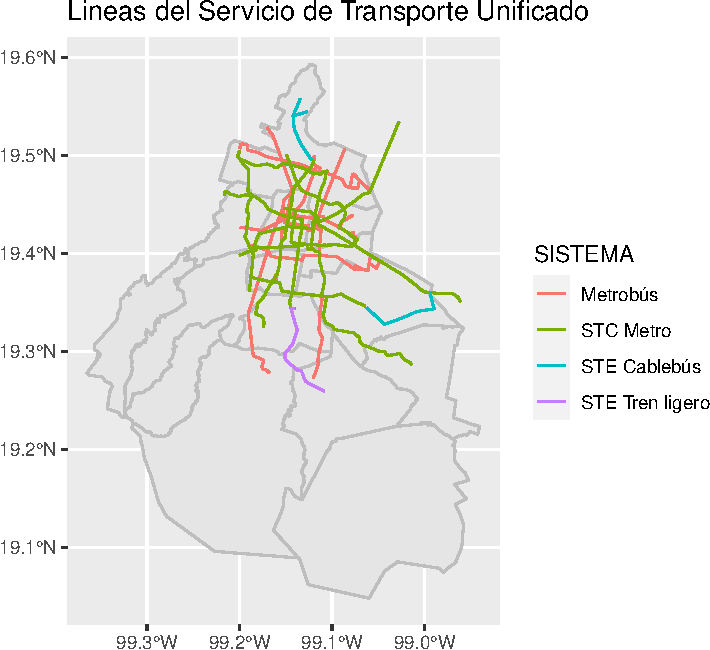
\includegraphics{proyecto_files/figure-latex/mapa-lineas-1} \end{center}

Como se puede ver en la figura, hay razón para sospechar que el
transporte público está concentrado al centro y norte del territorio, al
menos a primera vista y sin no se conoce bien la ciudad. La mayor
carencia aparente es al sur de la ciudad. En la figura
@ref(fig:mapa-alc) presentamos un mapa de la ciudad con divisiones
políticas para hacer más fácil referirnos a alcaldías específicas.

A partir de ahora nos referimos a la ``zona centro'' como la zona
comprendida por las alcaldías: Miguel Hidalgo, Cuauhtémoc, Benito
Juárez. Es precisamente esta zona en la que sospechamos está
sobre-concentrado el transporte público.

\begin{center}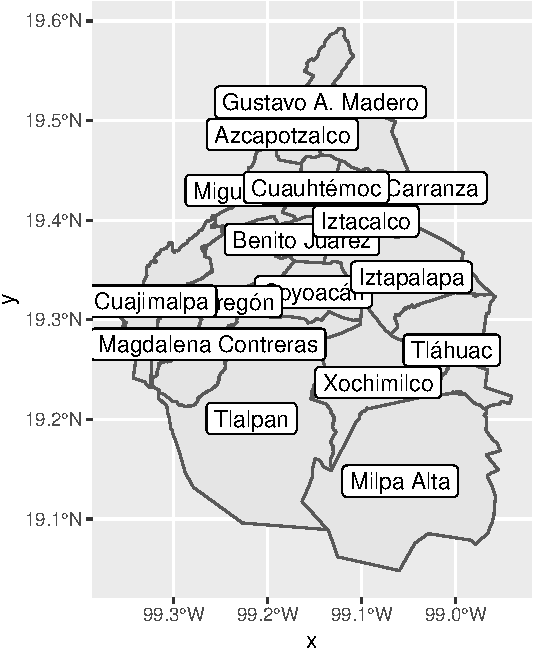
\includegraphics{proyecto_files/figure-latex/mapa-alc-1} \end{center}

Las carencias más grandes se pueden ver en las alcaldías de Tlalpan,
Magdalena Contreras, Xochimilco y Milpa Alta. A comparación de las
alcaldías al centro, las alcaldías en el sur tienen pocas estaciones,
pocas líneas, y una baja cobertura en general. Más tarde tomamos en
consideración la población y otros factores para comparar que tan fácil
es acceso de la población de una alcaldía al sistema de transporte
unificado. Uno de los factores clave para este análisis es la variable
que llamamos \texttt{MEAN\_DIST}: una métrica que utlizamos para medir
que tan fácil es el acceso de una alcaldía al transporte unificado, la
cual explicamos con más profundidad a continuación.

\hypertarget{distancia-promedio-al-transporte-puxfablico}{%
\subsubsection{Distancia promedio al transporte
público}\label{distancia-promedio-al-transporte-puxfablico}}

Para calcular una medida de acceso al transporte público nos pareció que
tomar solamente la cantidad de estaciones en total contenidas dentro de
los límites de una alcaldía sería muy insuficiente. Por ejemplo,
alcaldías como Cuajimalpa y Magdalena Contreras que no tienen ninguna
estación estarían efectivamente ``desconectadas'', pero eso no quiere
decir que sus habitantes no tengan manera alguna de transportarse.

Para estimar la ``conectividad'' tomamos información sobre el uso de
suelo de la CDMX publicado por la Secretaría de Desarrollo Urbano y
Vivienda \cite{usodesuelo}. Con esta información tomamos la localización
de todas las zonas registradas como habitacional o residencial
(e.g.~habitacional comercial, habitacional multifamiliar) y usando un
algoritmo conocido como BallTree calculamos a que distancia medida con
la métrica Haversine está de la estación de transporte unificado más
cercana. Asi obtenemos para cada zona residencial una distancia en
metros, y después calculamos la media para cada alcaldía para cada año.
Utilizamos esta información más tarde para hacer en análisis sobre
conectividad por población al que hacíamos referencia.

Decidimos calcularlo de esta manera para tener una mejor idea de cómo es
que el transporte está distribuido con respecto a la \emph{población} y
dónde vive ésta. Si tomáramos por ejemplo número total de estaciones
normalizado por área las alcaldías como Milpa Alta o Tlalpan mostrarían
un sesgo considerable dado que son muy grandes en términos de área pero
su población es mucho menor a otras alcaldías mucho más pequeñas.
Teniendo distancia promedio medida en metros con la métrica Haversine y
además la población podemos controlar tanto por el efecto de densidad
poblacional como el fenómeno de distribución de la misma. Para dar otro
ejemplo, si se tomara la distancia con los extremos de los límites de la
alcaldías veríamos que Cuajimalpa está peor conectado de el valor real.
¿Por qué? Porque por un extremo tenemos la zona Observatorio y por la
otra Desierto de los Leones. Desierto de los Leones está mucho más lejos
de la zona de cobertura del transporte, pero la población ahi es mucho
más pequeña que la de la zona Observatorio, por poner un ejemplo.

Vale la pena mencionar que una de las debilidades de este análisis es la
falta de información completa. En el conjunto de datos que se utilizó
para obtener la distancia promedio no hay ningún registro de las zonas
habitacionales para la alcaldía Álvaro Obregón, a pesar de que es una de
las más pobladas. Ignoramos la razón de esta falta de datos, pero es
razonable pensar que hay otras carencias que no se pueden distinguir a
simple vista y que podrían estar sesgando nuestro análisis.

\hypertarget{nuxfamero-total-de-estaciones-distancia-a-la-zona-centro}{%
\subsubsection{Número total de estaciones \& distancia a la zona
centro}\label{nuxfamero-total-de-estaciones-distancia-a-la-zona-centro}}

Para complementar nuestro análisis de conectividad utilizamos otras dos
variables calculadas a partir de los conjuntos de datos ya mencionados.
La primera de estas variables es el número total de estaciones de
transporte público unificado que se encuentran dentro de los límites de
una alcaldía dada para algún año fijo. Esto para tomar en cuenta cómo ha
evolucionado el sistema de transporte unificado.

La distancia a la zona centro se toma como la distancia promedio en la
métrica Haversine de las mismas zonas residenciales mencionadas en el
párrafo anterior al zócalo de la ciudad. Una vez más, se toma el
promedio de estas distancias para la alcaldía y el año correspondiente.

Reconocemos que la elección del zócalo de la ciudad como punto central
puede parecer arbitraria. Sin embargo, nos parece justificable puesto
que es una de las zonas más antiguas y por lo tanto el crecimiento de la
zona metropolitana de la ciudad ha sido radialmente hacia afuera de esta
zona. De manera similar, las primeras estaciones de metro y metrobus
fueron construidas precisamente para servir a la zona centro.

Con todas las variables a las que hicimos referencia podemos empezar el
análisis principal y el objetivo de este trabajo.

\hypertarget{acceso-a-transporte-con-base-en-la-poblaciuxf3n}{%
\subsection{Acceso a transporte con base en la
población}\label{acceso-a-transporte-con-base-en-la-poblaciuxf3n}}

Como se mostró antes, el mapa de líneas de transporte público unificado
muestra una concentración alta en la zona centro (alcaldías Cuauhtémoc,
Miguel Hidalgo y Benito Juárez). Esta concentración sería deseable si
éstas fueran las alcaldías más pobladas, ya que justamente una mayor
densidad poblacional justifica mayor inversión en el sistema. Con ayuda
de la figura {[}{]} podemos ver cómo es la distribución geográfica de la
población en la CDMX.

\begin{center}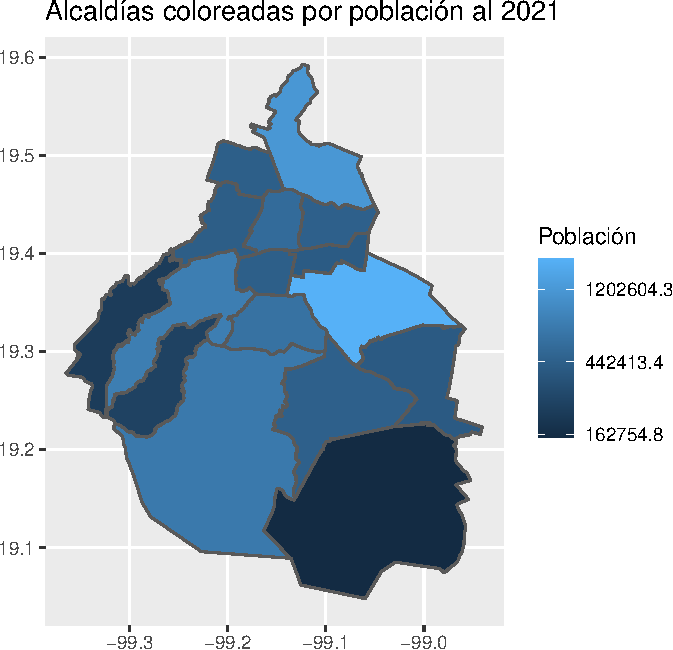
\includegraphics{proyecto_files/figure-latex/unnamed-chunk-6-1} \end{center}

Llama la atención que las alcaldías del centro efectivamente no son las
más pobladas. Las dos alcaldías más pobladas son Iztapalapa, Gustavo A.
Madero (GAM) y Álvaro Obregón. Tanto Iztapalapa como GAM están en la
periferia de la ciudad, y ninguna de las tres más pobladas está en la
``zona centro''.

En la figura {[}{]} vemos las alcaldías coloreadas dependiendo de
cuantas estaciones de transporte público al año 2021 tienen en total.

\begin{center}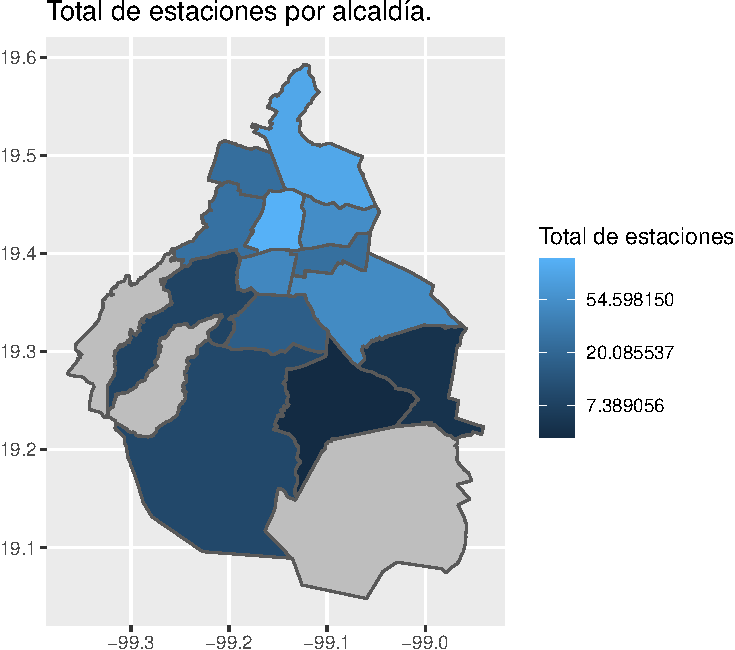
\includegraphics{proyecto_files/figure-latex/unnamed-chunk-7-1} \end{center}

Las alcaldías con el mayor número total de estaciones de transporte
público al año 2021 son Cuauhtémoc, GAM y Venustiano Carranza en ese
orden. De la lista de alcaldías más pobladas solo coinciden Gustavo A.
Madero. Notablemente Iztapalapa parece tener un déficit de transporte
público al ser la alcaldía más poblada por un margen alto, con más de 1
millón de habitantes, pero siendo la cuarta con más estaciones de
transporte público. También llama la atención que hay tres alcaldías que
no tienen una sola estación de transporte público: Cuajimalpa, Magdalena
Contreras y Milpa Alta. En el caso de Milpa Alta tiene sentido dada la
baja densidad poblacional, pero en Cuajimalpa no solo hay áreas
densamente pobladas, sino que hay áreas de suma importancia comercial
como la zona de Santa Fe.

Hasta el momento hemos tomado la información en el punto de tiempo más
reciente al que tenemos acceso: al año 2021. Para hacer un análisis más
robusto tomamos en cuenta el componente temporal y estudiamos cómo ha
cambiado la ``conectividad'' de diversas alcaldías con el paso del
tiempo.

En la figura {[}{]} se puede ver un \emph{boxplot} que ayuda a entender
la evolución de la conectividad como función del tiempo. En ella
comparamos las distancias promedio a la estación de transporte público
más cercano por alcaldía, donde cada observación corresponde a un año.
Dado que esta distancia es estrictamente decreciente (no se ha dado el
caso de que se elimine por completo una estación permanentemente), la
dispersión de los datos nos dice cómo se ha ido reduciendo esa distancia
desde que se creó la primera línea del metro hasta la actualidad.

Podemos ver que las alcaldías de Cuauhtémoc, Benito Juárez y Venustiano
Carranza tienen las menores varianzas en distancia media y además las
más pequeñas. Estas alcaldías son precisamente la que definimos como
``zona centro'' desde el inicio. De esta observación confirmamos que la
zona centro siempre ha estado muy bien conectada porque el sistema de
transporte unificado fue construido pensando en servir específicamente a
esta zona. Además, se puede notar que su distancia promedio promedio a
la estación de transporte más cercana sigue siendo muy baja en
comparación a otras alcaldías, incluso las más pobladas como Iztapalapa.

Por otro lado, Tláhuac, Cuajimalpa y Milpa Alta son los de mayor
distancia y variación. En el caso de Tlahuac por ejemplo, siendo una de
las alcaldías más al sur, lo que interpretamos es que su distancia
promedio a las primeras estaciones era excesivamente alta y fue
disminuyendo a medida que mejoró la cobertura. En el cao de Cuajimalpa
la distancia disminuyó dramáticamente pero al día de hoy, sigue siendo
la alcaldía ``peor conectada'' por distancia.

Otra cosa que podemos observar es que la línea en la caja que marca la
media está en todos los caso mucho más cerca del extremo izquierdo de la
caja. Lo cual nos quiere decir que los datos están sesgados, y que la
mayoría está más cerca del lado de ``distancia baja''. En otras
palabras, la distancia promedio mejoró muy rápidamente, lo cual sugiere
que el sistema de transporte unificado evolucionó rápidamente para
cubrir gran parte de la zona metropolitana.

\begin{center}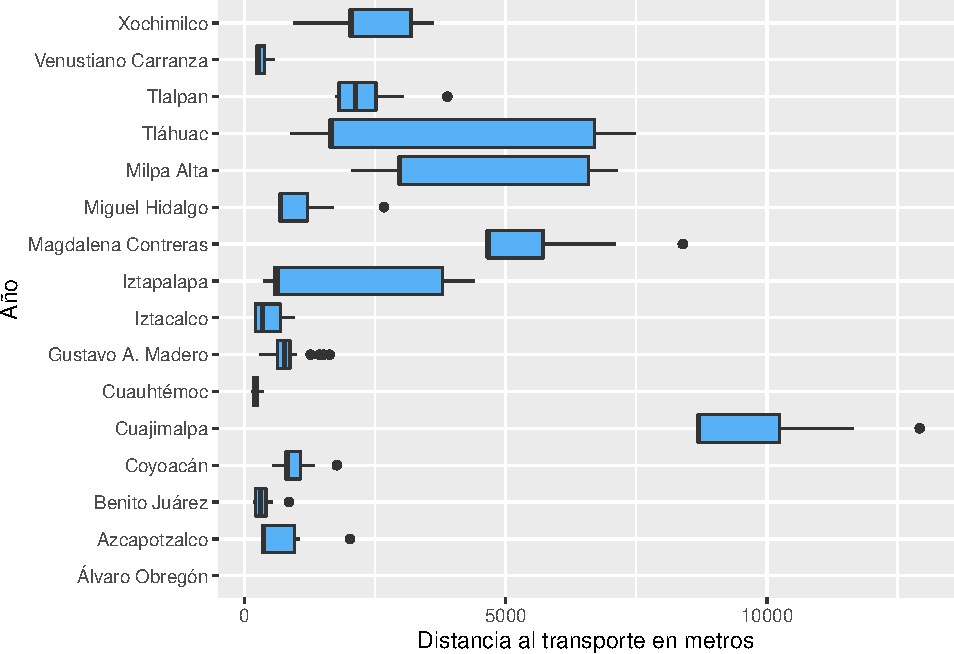
\includegraphics{proyecto_files/figure-latex/unnamed-chunk-8-1} \end{center}

\begin{center}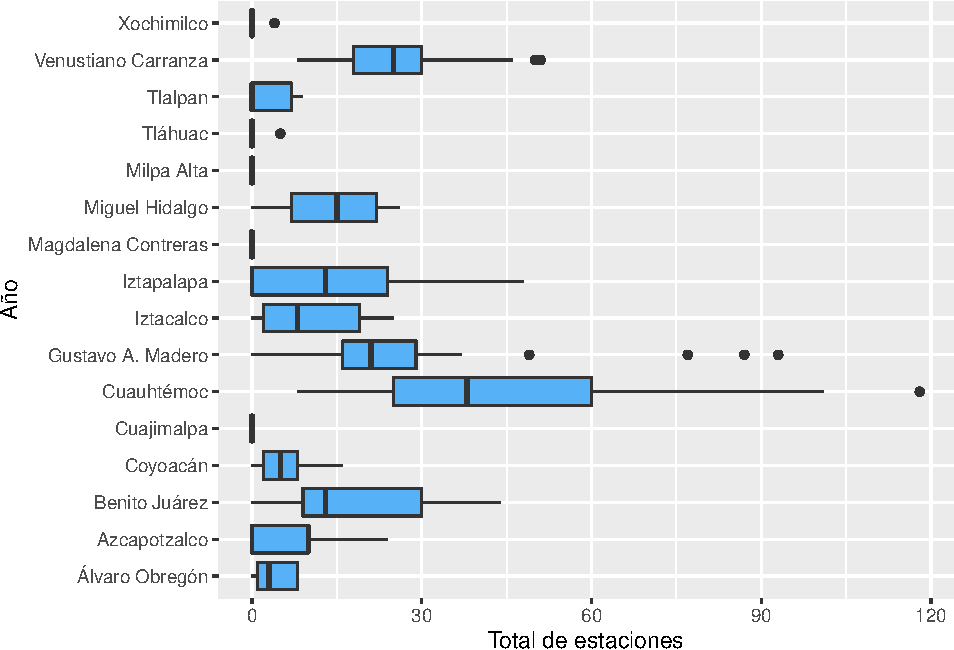
\includegraphics{proyecto_files/figure-latex/unnamed-chunk-8-2} \end{center}

\begin{center}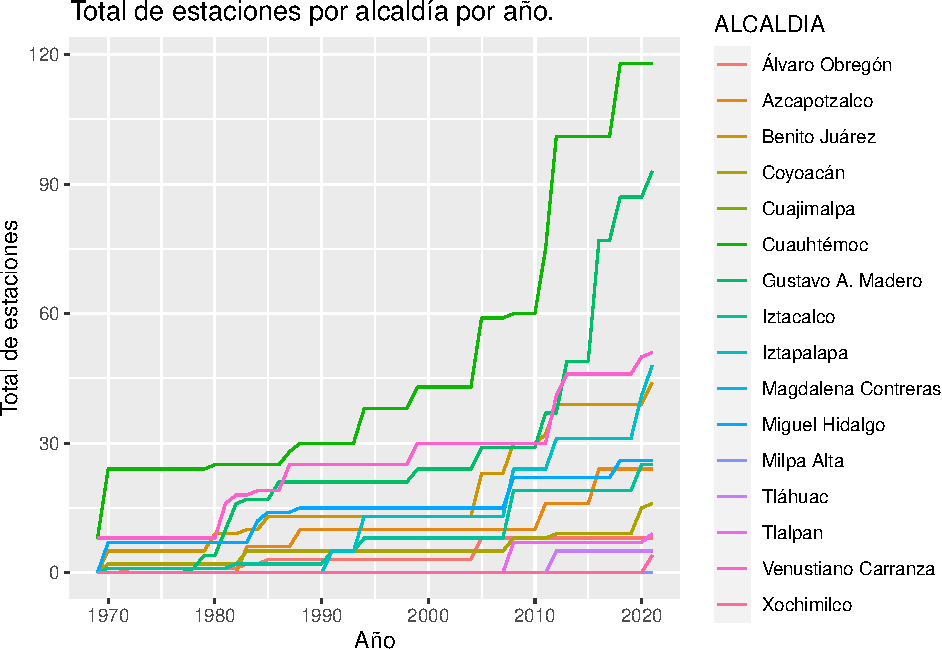
\includegraphics{proyecto_files/figure-latex/unnamed-chunk-9-1} \end{center}

En la figura {[}{]} consideramos el número total de estaciones en la
alcaldía como función del tiempo. Aqui podemos ver que el número de
estaciones en las alcadías de la zona centro excede vastamente el de las
alcaldías más periféricas, como Iztapalapa. Analizando la variabilidad
mediante el ancho de la caja podemos ver también que por ejemplo en la
alcaldía Cuauhtémoc y GAM se han construido muchas estaciones con el
paso de los años. Lo cual nos da pistas por ejemplo en el caso de
Cuauhtémoc que no solo comenzaron estando muy bien conectadas, la
inversión ha continuado más y más a pesar de que era buena desde un
inicio. El número total de estaciones en Cuauhtémoc ha llegado a casi
120, mientras que en la mayoría no se exceden las 50.

Otra cosa que llama la atención es el caso de Benito Juárez. El número
total de estaciones no ha crecido tan dramáticamente como en las otras
alcaldías de la zona centro, pero recordando su distancia promedio al
transporte es una de las alcaldías mejor conectadas. Esto nos indica que
a pesar de que no se han hecho muchas estaciones nuevas en sus límites
territoriales, las que se han hecho han estado en la zona circundante y
han mejorado su conectividad. Esa zona es precisamente la zona centro.
Una pista más que indica que la inversión en creación de nuevas líneas
ha estado privilegiando a la zona centro.

\hypertarget{anuxe1lisis-de-correlaciuxf3n}{%
\subsubsection{Análisis de
Correlación}\label{anuxe1lisis-de-correlaciuxf3n}}

Si bien hasta ahora nos hemos servido de interpretar diversas gráficas
para tomar intuición, si queremos cuantificar qué tan notorio es el
efecto de inversión privilegiada en la zona centro tenemos que servirnos
de otras técnicas estadísticas. Por ejemplo, si nuestra hipótesis tiene
evidencia favorable esperaríamos observar una correlación positiva entre
distancia al zócalo de la ciudad y la conectividad medida como distancia
promedio al transporte más cercano y número total de estaciones. En la
figura {[}{]} vemos un diagrama de correlación para las variables
estudiadas.

\begin{center}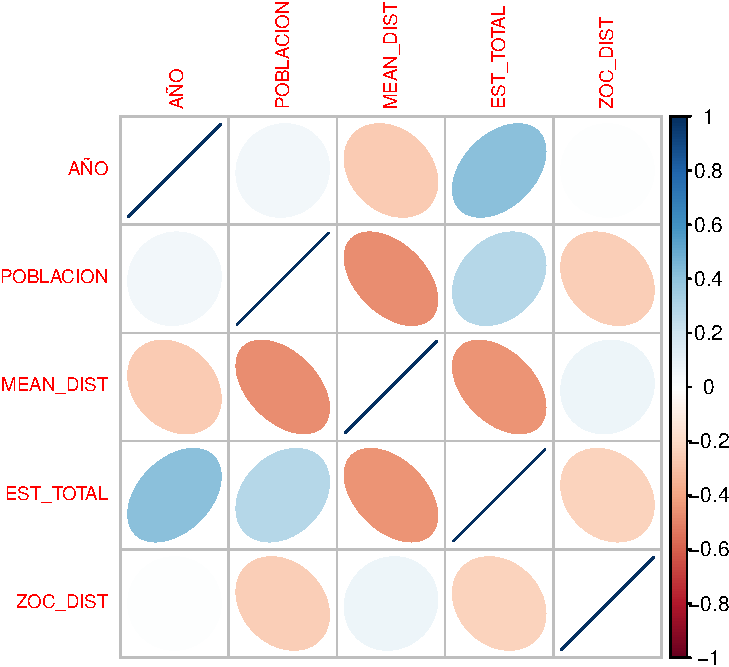
\includegraphics{proyecto_files/figure-latex/unnamed-chunk-10-1} \end{center}

Efectivamente se cumple que la correlación de distancia al Zocalo con
distancia al transporte más cercano es positiva. Es decir, entre más se
aleja la zona habitacional del zócalo, más se aleja de la zona de
cobertura del sistema de transporte unificado. También se puede apreciar
este fenómeno en la correlación negativa entre distancia al zócalo con
el número total de estaciones. Es decir, entre más lejos está la
alcaldía del zócalo menor es el número total de estaciones a las que se
tiene acceso. Las correlaciones son aparentemente débiles, pero
notables. Sospechamos que la correlación se hace más fuerte a medida que
se va hacia atrás en el tiempo cuando había menos estaciones en total.
El corolario es que esta conectividad si ha estado mejorando desde que
se empezó a construir la primera linea de metro hasta la actualidad.

La matriz explícita de correlaciones es:

\begin{table}

\caption{\label{tab:unnamed-chunk-11}Matriz de correlación entre las variables de interés.}
\centering
\begin{tabular}[t]{lrrrrr}
\toprule
  & AÑO & POBLACION & MEAN\_DIST & EST\_TOTAL & ZOC\_DIST\\
\midrule
AÑO & 1.000 & 0.050 & -0.253 & 0.411 & 0.000\\
POBLACION & 0.050 & 1.000 & -0.461 & 0.290 & -0.249\\
MEAN\_DIST & -0.253 & -0.461 & 1.000 & -0.443 & 0.077\\
EST\_TOTAL & 0.411 & 0.290 & -0.443 & 1.000 & -0.222\\
ZOC\_DIST & 0.000 & -0.249 & 0.077 & -0.222 & 1.000\\
\bottomrule
\end{tabular}
\end{table}

Si graficamos la distancia promedio al sistema de transporte por
alcaldía la correlación espacial entre distancia al centro de la ciudad
aproximado mediante la posición del zócalo podremos tener indicación
visual de si nuestra hipótesis tiene sentido. Como medida de
visualización está bien, pero hay varios problemas con ella como método
formal. Por ejemplo, que algunas alcaldías son muy ``largas'' y sus
puntos más cercanos y más lejanos el centro de la ciudad serán
coloreados del mismo color a pesar de que no tienen la misma
conectividad. El mejor ejemplo de este caso es Álvaro Obregón. Su zona
norte y oriente están bien conectadas: cerca de Tacubaya y con el
corredor Insurgentes Sur respectivamente. Por otro lado, las zonas como
Los Dínamos y Las Águilas están muy lejos del resto del sistema.

\begin{center}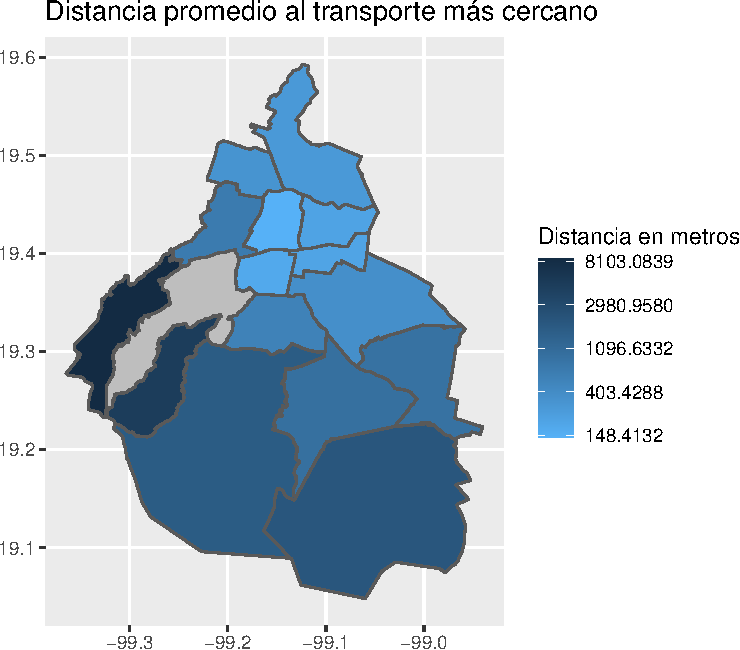
\includegraphics{proyecto_files/figure-latex/unnamed-chunk-12-1} \end{center}

Ahora vemos cómo evoluciona como función del tiempo.

\begin{center}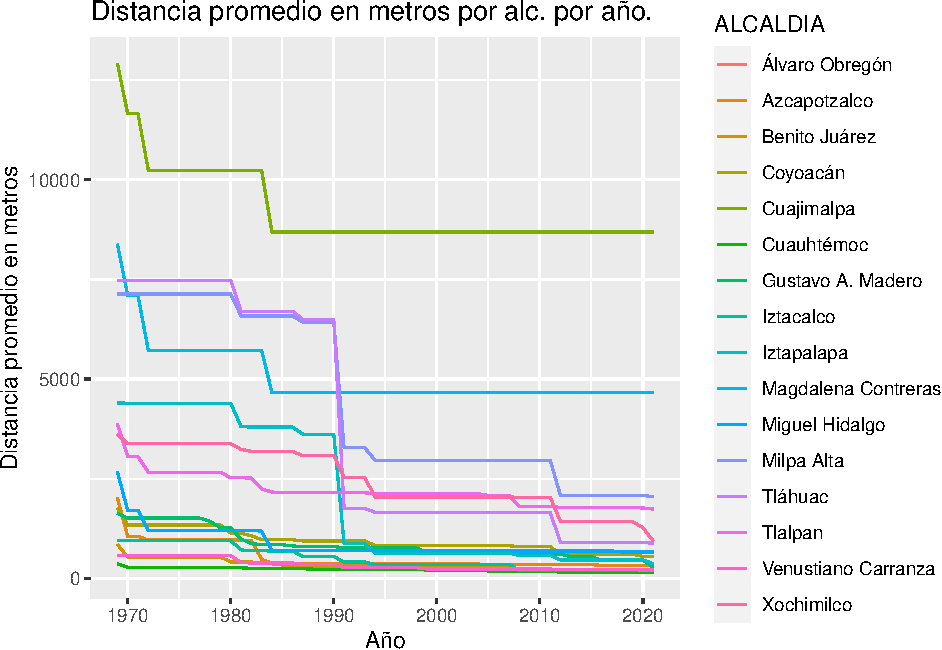
\includegraphics{proyecto_files/figure-latex/unnamed-chunk-13-1} \end{center}

\begin{center}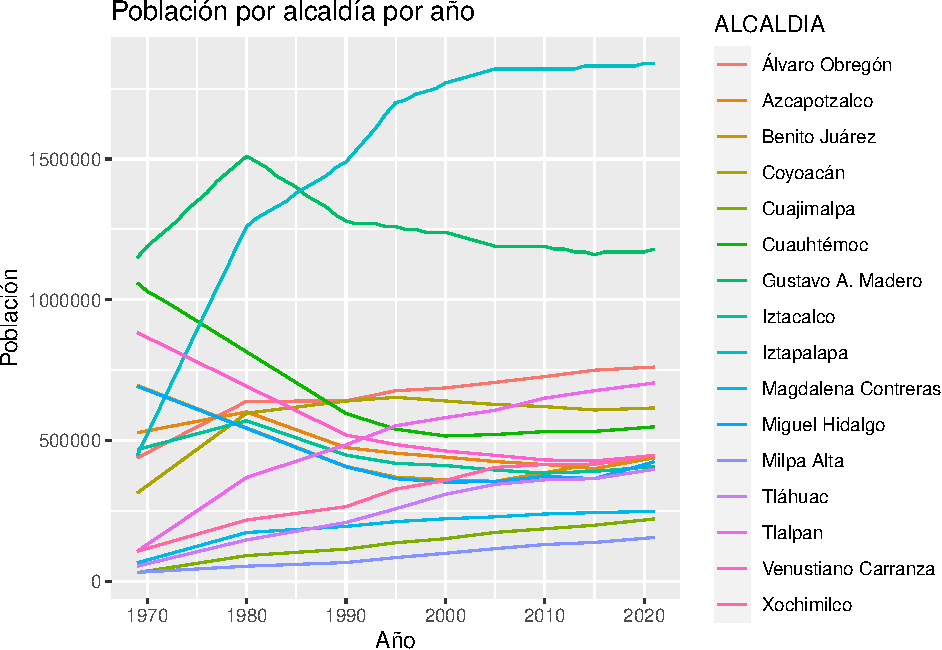
\includegraphics{proyecto_files/figure-latex/unnamed-chunk-14-1} \end{center}

\hypertarget{pca}{%
\section{PCA}\label{pca}}

\begin{verbatim}
## 
## Loadings:
##           Comp.1 Comp.2 Comp.3 Comp.4 Comp.5
## AÑO        0.363  0.643  0.327  0.581  0.105
## POBLACION  0.462 -0.434 -0.400  0.496 -0.438
## MEAN_DIST -0.536         0.450  0.239 -0.672
## EST_TOTAL  0.547  0.195  0.231 -0.597 -0.503
## ZOC_DIST  -0.262  0.599 -0.691        -0.303
## 
##                Comp.1 Comp.2 Comp.3 Comp.4 Comp.5
## SS loadings       1.0    1.0    1.0    1.0    1.0
## Proportion Var    0.2    0.2    0.2    0.2    0.2
## Cumulative Var    0.2    0.4    0.6    0.8    1.0
\end{verbatim}

\begin{center}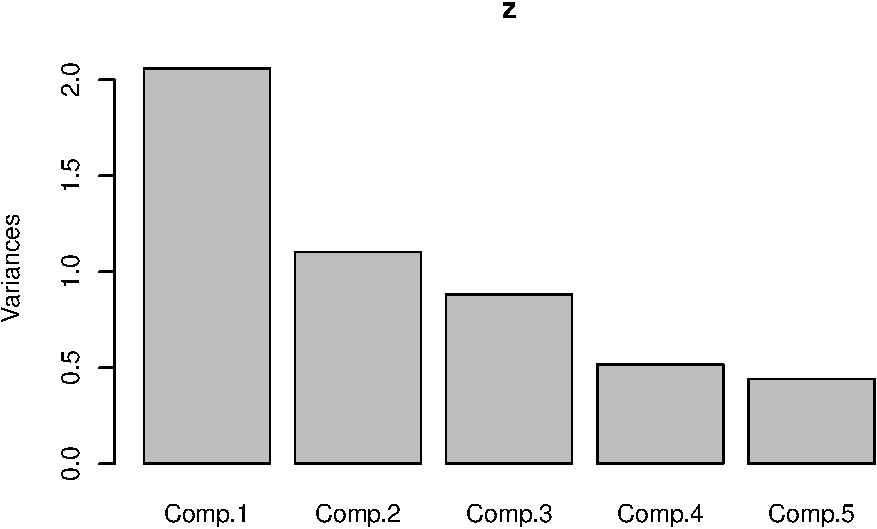
\includegraphics{proyecto_files/figure-latex/unnamed-chunk-16-1} \end{center}

\hypertarget{construcciuxf3n-de-un-uxedndice-de-conectividad}{%
\section{Construcción de un índice de
conectividad}\label{construcciuxf3n-de-un-uxedndice-de-conectividad}}

Aquí construimos un índice de conectividad basado en los datos del año
2021. El índice lo construimos por medio del análisis factorial. Las
variables utilizadas serán la distancia promedio a las estaciones y
cantidad de estaciones en la alcaldía. La prueba de esfericidad de
Bartlett indica que las correlaciones son significativas ya que
aplicarla da un valor-\(p\) de \ensuremath{2.4702932\times 10^{-22}} y
la prueba Kaiser--Meyer--Olkin (KMO) indica una adecuación medianamente
regular. El valor es de 0.5, es apenas suficiente para justificar el uso
de esta técnica.

El gráfico de sedimentación (scree plot en inglés) indica que un factor
es suficiente en este caso.

\begin{center}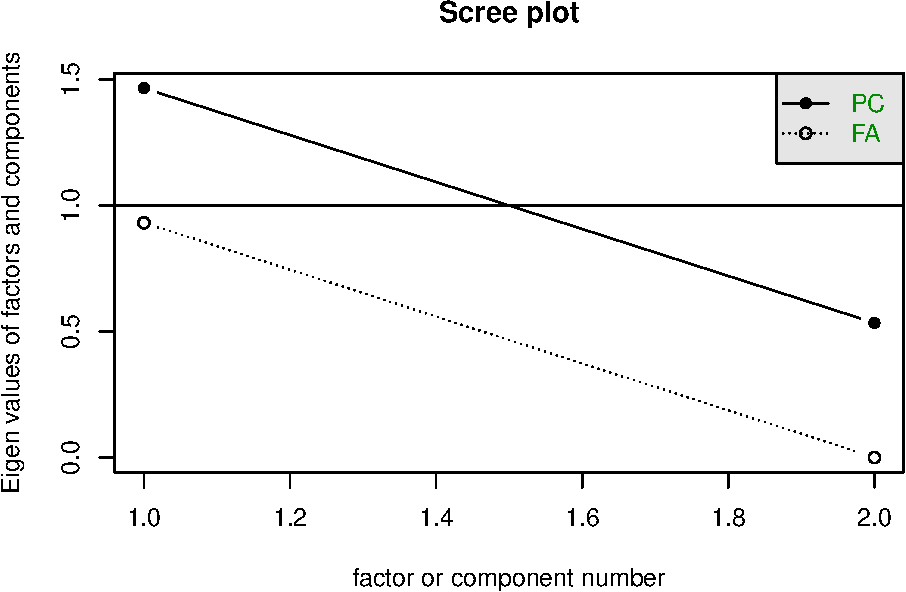
\includegraphics{proyecto_files/figure-latex/unnamed-chunk-20-1} \end{center}

Queremos combinar la información que dan el número total de estaciones y
la distancia promedio a ellas para aproximar una variable intangible:
qué tan conectada está la alcaldía al resto del sistema de transporte
público unificado. Para esto utilizamos análisis de factores para
construir un índice de conectividad. En la tabla \ref{fig:fa-output} (en
el apéndice \ref{sec:fig-omitidas}) se puede encontrar la salida
completa de la aplicación de esta función al conjunto de datos. El
diagrama que explica cómo está construido el índice y la participación
de cada factor que lo compone se puede ver en la figura
\ref{fig:diagrama}.

Al ver el modelo generado, vemos que el factor o constructo da
importancias comparables a la cantidad total de estaciones de transporte
en la alcaldía como su distancia promedio a ellas. Un valor muy alto del
índice indicaría que hay muy buen acceso en cuanto a número de
estaciones, las cuales están bien distribuidas en el territorio lo cual
baja la distancia promedio a ellas. Un índice bajo indica que no solo no
hay muchas o ninguna estación en el territorio, las más cercanas en
otras alcaldías están relativamente lejos.

\begin{verbatim}
## Factor Analysis using method =  ml
## Call: fa(r = df2, nfactors = 1, rotate = "varimax", fm = "ml")
## Standardized loadings (pattern matrix) based upon correlation matrix
##             ML1   h2   u2 com
## EST_TOTAL -0.68 0.47 0.53   1
## MEAN_DIST  0.68 0.47 0.53   1
## 
##                 ML1
## SS loadings    0.93
## Proportion Var 0.47
## 
## Mean item complexity =  1
## Test of the hypothesis that 1 factor is sufficient.
## 
## The degrees of freedom for the null model are  1  and the objective function was  0.24 with Chi Square of  3.06
## The degrees of freedom for the model are -1  and the objective function was  0 
## 
## The root mean square of the residuals (RMSR) is  0 
## The df corrected root mean square of the residuals is  NA 
## 
## The harmonic number of observations is  15 with the empirical chi square  0  with prob <  NA 
## The total number of observations was  15  with Likelihood Chi Square =  0  with prob <  NA 
## 
## Tucker Lewis Index of factoring reliability =  1.528
## Fit based upon off diagonal values = 1
## Measures of factor score adequacy             
##                                                    ML1
## Correlation of (regression) scores with factors   0.80
## Multiple R square of scores with factors          0.64
## Minimum correlation of possible factor scores     0.27
\end{verbatim}

\begin{center}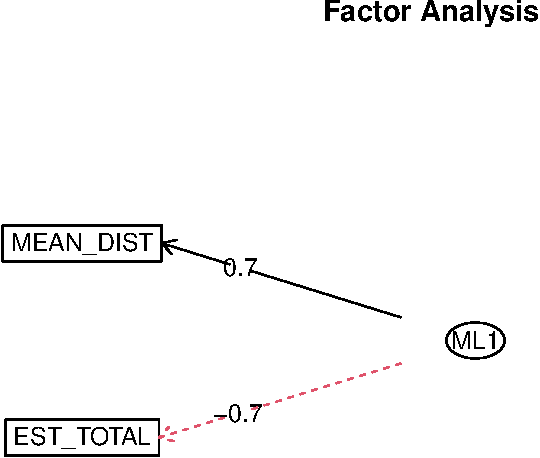
\includegraphics{proyecto_files/figure-latex/unnamed-chunk-21-1} \end{center}

Construimos ahora el índice para cada delegación en 2021. Podemos ver
que las delegaciones con el índice más alto coinciden con las
delegaciones con más estaciones y más población, que son las de la zona
centro e Iztapalapa.

\begin{table}

\caption{\label{tab:unnamed-chunk-23}Índice de conectividad calculado al 2021.}
\centering
\begin{tabular}[t]{lr}
\toprule
  & ML1\\
\midrule
Cuauhtémoc & 1.000\\
Gustavo A. Madero & 0.891\\
Venustiano Carranza & 0.725\\
Iztapalapa & 0.704\\
Benito Juárez & 0.699\\
Iztacalco & 0.621\\
Azcapotzalco & 0.609\\
Miguel Hidalgo & 0.597\\
Coyoacán & 0.564\\
Tláhuac & 0.499\\
Xochimilco & 0.491\\
Tlalpan & 0.462\\
Milpa Alta & 0.407\\
Magdalena Contreras & 0.247\\
Cuajimalpa & 0.000\\
\bottomrule
\end{tabular}
\end{table}

\begin{center}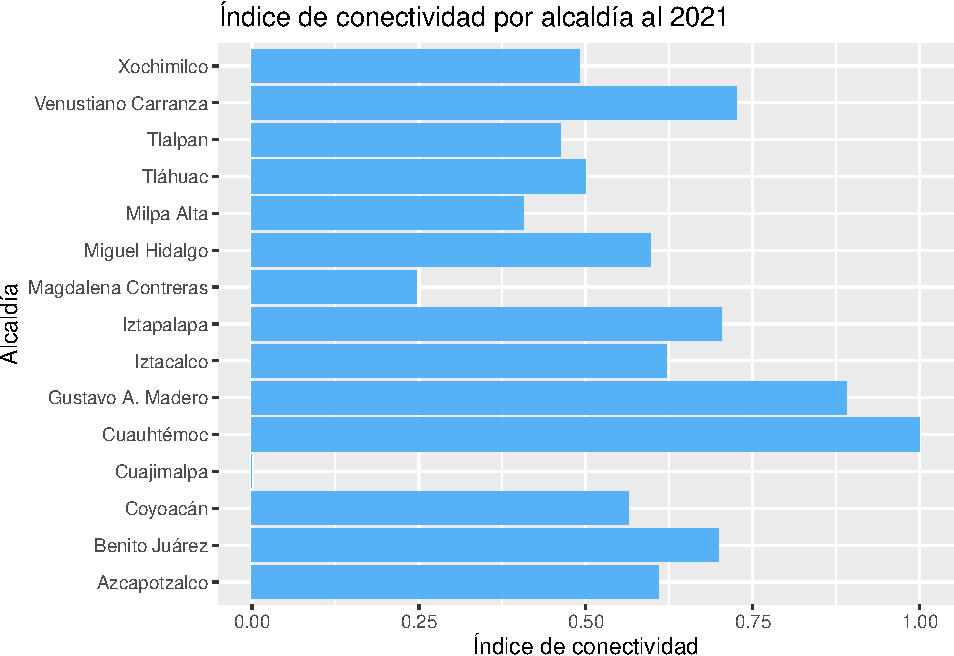
\includegraphics{proyecto_files/figure-latex/unnamed-chunk-24-1} \end{center}

\begin{center}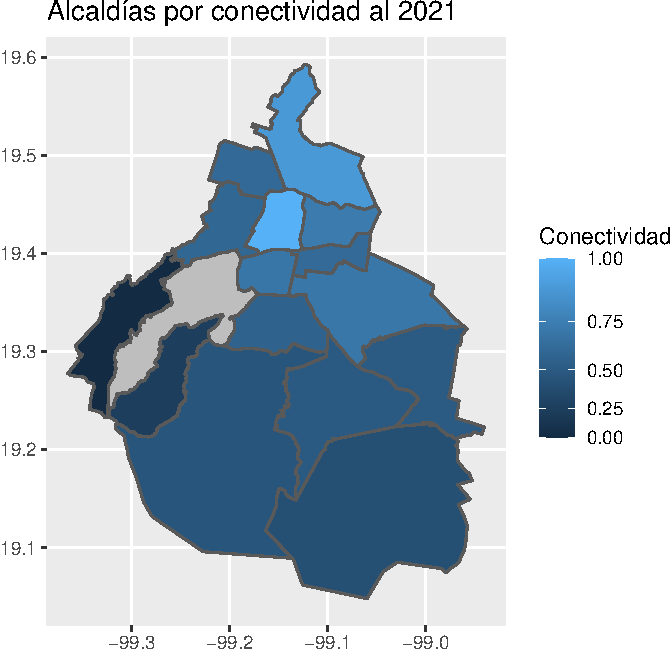
\includegraphics{proyecto_files/figure-latex/unnamed-chunk-25-1} \end{center}

\hypertarget{anuxe1lisis-del-uxedndice-de-conectividad-por-auxf1o}{%
\subsection{Análisis del índice de conectividad por
año}\label{anuxe1lisis-del-uxedndice-de-conectividad-por-auxf1o}}

El mapa nos ayuda a identificar patrones espaciales, pero para notar
patrones temporales utilizamos \textit{boxplots}, también conocidas como
gráficas de caja y bigotes. Lo que ellas nos permiten es ver mediante su
largo cómo es que ha cambiado la variable a través del tiempo. Por
ejemplo un \textit{boxplot} muy largo indica mucha variación, o en otras
palabras, si nos concentramos en la figura \ref{fig:est_tot-v-ano}, en
el caso de Cuauhtémoc vemos que su caja es de las más largas. De esto
inferimos que es donde más se han construido estaciones, ya que pasó de
tener relativamente pocas a tener la mayor cantidad. Cuajimalpa por
ejemplo tiene un punto en vez de caja porque en todos los años ha tenido
la misma cantidad de estaciones: ninguna.

\begin{center}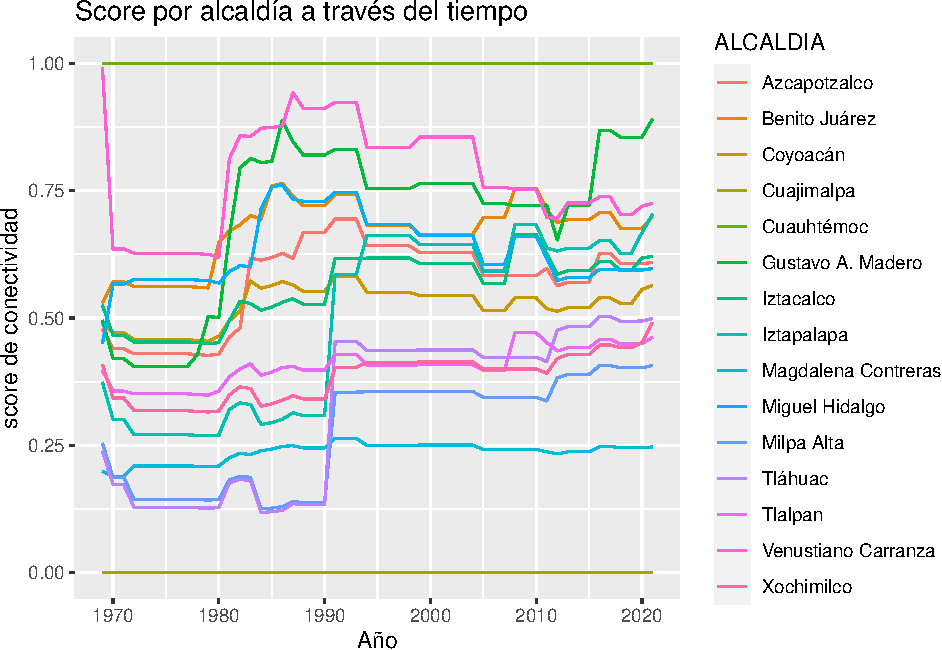
\includegraphics{proyecto_files/figure-latex/unnamed-chunk-27-1} \end{center}

\begin{center}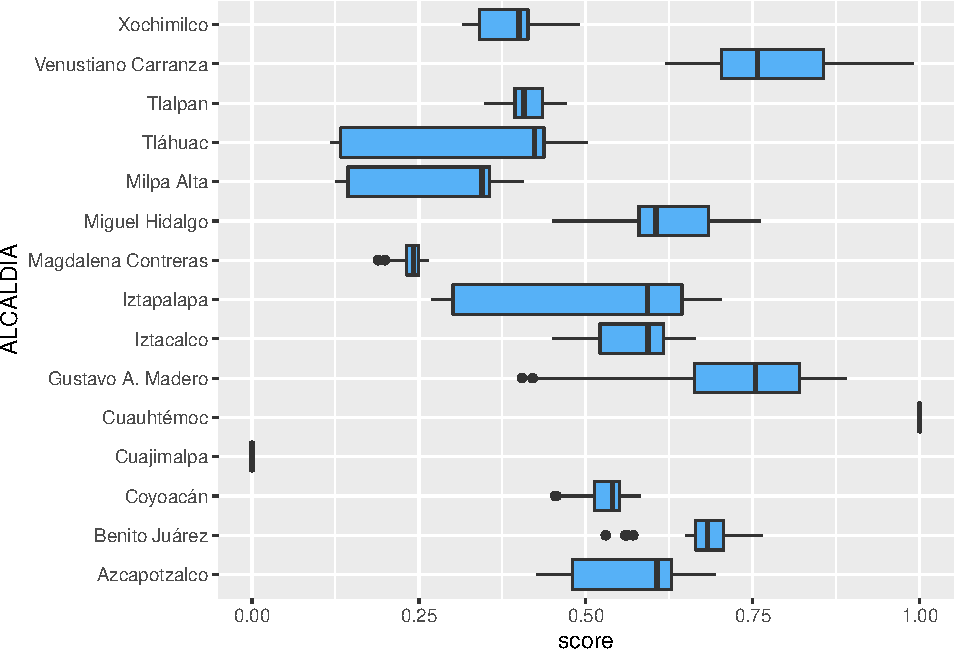
\includegraphics{proyecto_files/figure-latex/unnamed-chunk-28-1} \end{center}

Otra ventaja de utilizar boxplots para analizar la dinámica es que tanto
el total de estaciones como la distancia a ellas son funciones
monótonas: el número de estaciones no se disminuye porque no se
destruyen líneas (exceptuando el caso extraordinario de la línea dorada)
y la distancia promedio a estaciones no aumenta por la misma razón.
Entonces, el sesgo de los datos nos ayuda a entender en qué punto de
tiempo se construyeron las estaciones que conllevan a los cambios en las
variables. Que la línea que indica la media de los datos esté sesgada a
la izquierda nos indica que en la mayoría de observaciones (es decir
años), por ejemplo, el total de estaciones ha sido bajo y que este
aumentó recientemente. Un sesgo a la derecha indica lo contrario: que el
número de estaciones creció relativamente temprano en esta ventana de
tiempo que estamos estudiando, y la mayoría de los años desde 1969 a la
fecha los ha experimentado con esa cantidad alta de estaciones.

En ejemplos concretos, en la figura \ref{fig:dist-v-ano} el extremo
sesgo que se puede ver en la caja de Cuajimalpa nos indica que su
distancia promedio al transporte mejoró apenas recientemente, y que en
la ventana de tiempo estudiada la mayoría del transporte se constuyó
lejos de Cuajimalpa. Lo mismo para Iztapalapa, que como ya discutimos
mejoró mucho gracias a la construcción de la línea morada y del
cablebus. La linea morada se construyó en 1991 y el cablebus en 2021,
ambos en la segunda mitad del periodo de tiempo sobre el cual tenemos
datos.

Para tener mejor idea sobre en que años específicamente se dieron los
cambios que dieron lugar a los cambios en la conectividad presentamos en
la figura \ref{fig:idx-v-tiempo} la gráfica del índice de conectividad
con respecto al tiempo. En ella vemos una vez más los cambios drásticos
que ya habíamos comentado respecto a Iztapalapa, Milpa Alta y Tláhuac:
el extremo oriente de la ciudad. Damos crédito a esta mejora dramática
en conectividad a la linea morada del metro que mejora muchísimo la
distancia promedio a la estación de transporte más cercana.

Otra cosa interesante que podemos notar es que a pesar de que tanto el
número total de estaciones como la distancia promedio a ellas son
monótonas el índice si sube y baja. Esto se debe a que este score de
conectividad empeora cuando el de otras alcaldías mejora, como se puede
ver por ejemplo con Azcapotzalco a principios de la década de 1990.

\hypertarget{regresiuxf3n-lineal}{%
\section{Regresión lineal}\label{regresiuxf3n-lineal}}

Para interpretar el papel que juega la población en el incremento de
conectividad de una alcaldía utilizamos un modelo lineal por sus
propiedades de interpretación. Estimamos el siguiente modelo:
\begin{equation}
\text{score}_i = \log(\text{AÑO}_i) + \log(\text{POBLACION}_i) + \varepsilon_i,
\end{equation} al conjunto de datos que de todas las alcaldías
disponibles salvo Álvaro Obregón ya que no se pudo calcular el índice
por la falta de datos, ni Cuauhtémoc ni Cuajimalpa porque su índice es
siempre 1 y 0 respectivamente lo cual causa problemas en la estimación.

Para poder utilizar el modelo primero verificamos que se cumplan sus
supuestos: homocedasticidad, no autocorrelación y rango completo. Para
eso usamos las pruebas de White, Breusch--Godfrey y el valor
inflacionario de la varianza que prueban por cada supuesto
respectivamente. Los resultados de aplicar dichas pruebas se pueden
encontrar en la siguiente tabla:

\begin{tabular}{lr}
\toprule
Prueba & valor\_p\\
\midrule
White & 0.000\\
Breusch--Godfrey & 0.000\\
máx VIF & 1.024\\
\bottomrule
\end{tabular}

Para las pruebas de White y Breusch--Godfrey la hipótesis nula es
homocedasticidad y no autocorrelación respectivamente. El VIF (valor
inflacionario de la varianza) se usa como regla de decisión, si está por
debajo de 30 no hay problemas graves de multicolinealidad. Como se puede
ver, los valores-\(p\) son ceros numéricos, por lo que no se rechaza la
hipótesis nula y se cumplen tanto homocedasticidad como no
autocorrelación. Por el otro lado, como el valor VIF más grande es
apenas mayor a 1, no tenemos ningún problema de multicolinealidad. En
resumen: se puede aplicar el modelo y usar los resultados para dar
conclusiones estadísticas.

Los coeficientes estimados son:

\% Table created by stargazer v.5.2.3 by Marek Hlavac, Social Policy
Institute. E-mail: marek.hlavac at gmail.com \% Date and time: mié, jun
08, 2022 - 14:59:08 \% Requires LaTeX packages: dcolumn

\begin{table}[!htbp] \centering 
  \caption{Estimación de parámetros para modelo lineal descrito.} 
  \label{} 
\begin{tabular}{@{\extracolsep{5pt}}lD{.}{.}{-3} } 
\\[-1.8ex]\hline 
\hline \\[-1.8ex] 
 & \multicolumn{1}{c}{\textit{Dependent variable:}} \\ 
\cline{2-2} 
\\[-1.8ex] & \multicolumn{1}{c}{log(score)} \\ 
\hline \\[-1.8ex] 
 log(AÑO) & 3.617^{***}$ $(0.484) \\ 
  log(POBLACION) & 0.098^{***}$ $(0.005) \\ 
  Constant & -27.672^{***}$ $(3.674) \\ 
 \hline \\[-1.8ex] 
Observations & \multicolumn{1}{c}{689} \\ 
R$^{2}$ & \multicolumn{1}{c}{0.446} \\ 
Adjusted R$^{2}$ & \multicolumn{1}{c}{0.445} \\ 
Residual Std. Error & \multicolumn{1}{c}{0.096 (df = 686)} \\ 
F Statistic & \multicolumn{1}{c}{276.483$^{***}$ (df = 2; 686)} \\ 
\hline 
\hline \\[-1.8ex] 
\textit{Note:}  & \multicolumn{1}{r}{$^{*}$p$<$0.1; $^{**}$p$<$0.05; $^{***}$p$<$0.01} \\ 
\end{tabular} 
\end{table}

Se puede ver que los coeficientes asociados a cada variable son
altamente significativos. Tanto el año como la población de una alcaldía
se relacionan positivamente con su nivel de conectividad, pero el
coeficiente asociado al año es mucho mayor. Eso nos indica que si el
gobierno continúa desarrollando transporte público al mismo paso se
espera que la conectividad de cada alcaldía mejore notablemente,
mientras que la población casi no explica el aumento en la oferta de
transporte público para una alcaldía dada.

Finalmente llevamos a cabo este mismo análisis, pero ajustando este
modelo sobre el conjunto de datos restringido a una sola alcaldía para
cada alcaldía. La tabla que contiene todos los coeficientes estimados se
puede econtrar en los anexos, por ahora solo mencionamos ejemplos
notables. Entre estos destacan Milpa Alta y GAM.

\begin{table}

\caption{\label{tab:unnamed-chunk-33}Coeficientes del modelo estimado para GAM y Milpa Alta.}
\centering
\begin{tabular}[t]{llrrrl}
\toprule
ALCALDIA & term & estimate & std.error & p.value & is.signif\\
\midrule
Gustavo A. Madero & (Intercept) & -88.973 & 13.503 & 0.000 & signif\\
Gustavo A. Madero & log(AÑO) & 11.378 & 1.668 & 0.000 & signif\\
Gustavo A. Madero & log(POBLACION) & 0.426 & 0.166 & 0.013 & signif\\
\addlinespace
Milpa Alta & (Intercept) & -49.473 & 50.868 & 0.335 & no signif\\
Milpa Alta & log(AÑO) & 6.515 & 6.759 & 0.340 & no signif\\
Milpa Alta & log(POBLACION) & 0.049 & 0.112 & 0.663 & no signif\\
\bottomrule
\end{tabular}
\end{table}

Para GAM todos los coeficientes son altamente significativos, y el
coeficiente asociado a la población es mucho más grande comparado al
modelo de todas las alcaldías en conjunto. Por el otro lado, para Milpa
Alta ningún coeficiente es significativo al 10\%, lo cual da pistas de
que lo que pase en Milpa Alta es de poco interés para las autoridades
encargadas de planear y construir transporte público, lo cual no
sorprende dada su baja densidad poblacional.

Usando técnicas se regresión lineal podríamos ajustar este modelo a
diferentes subconjuntos de datos: las alcaldías del centro y el resto.
Asi podríamos analizar si los coeficientes son significativamente
diferentes. Sin embargo, en interés de la brevedad no incluímos este
análisis final.

\hypertarget{interpretaciuxf3n-conclusiones-etc}{%
\section{Interpretación, conclusiones,
etc\ldots{}}\label{interpretaciuxf3n-conclusiones-etc}}

\hypertarget{apuxe9ndices}{%
\section{Apéndices}\label{apuxe9ndices}}

\hypertarget{coeficientes-de-la-regresiuxf3n-segmentada-por-alcalduxeda}{%
\subsection{Coeficientes de la regresión segmentada por
alcaldía}\label{coeficientes-de-la-regresiuxf3n-segmentada-por-alcalduxeda}}

A continuación la tabla a la que se hace referencia en la sección de
regresión lineal. Contiene los coeficientes estimados para el modelo
presentado para cada alcaldía junto con su error estándar, valor-\(p\),
y si es o no significativa a un nivel de 10\%.

\begin{table}

\caption{\label{tab:unnamed-chunk-34}Coeficientes estimados por alcaldía con significancia al 10 por ciento.}
\centering
\begin{tabular}[t]{llrrrl}
\toprule
ALCALDIA & term & estimate & std.error & p.value & is.signif\\
\midrule
Azcapotzalco & (Intercept) & 4.840 & 14.848 & 0.746 & no signif\\
Azcapotzalco & log(AÑO) & -0.335 & 1.872 & 0.859 & no signif\\
Azcapotzalco & log(POBLACION) & -0.299 & 0.110 & 0.009 & signif\\
\addlinespace
Benito Juárez & (Intercept) & -1.180 & 5.614 & 0.834 & no signif\\
Benito Juárez & log(AÑO) & 0.329 & 0.722 & 0.651 & no signif\\
Benito Juárez & log(POBLACION) & -0.132 & 0.027 & 0.000 & signif\\
\addlinespace
Coyoacán & (Intercept) & -3.028 & 3.211 & 0.350 & no signif\\
Coyoacán & log(AÑO) & 0.376 & 0.433 & 0.389 & no signif\\
Coyoacán & log(POBLACION) & 0.093 & 0.019 & 0.000 & signif\\
\addlinespace
Gustavo A. Madero & (Intercept) & -88.973 & 13.503 & 0.000 & signif\\
Gustavo A. Madero & log(AÑO) & 11.378 & 1.668 & 0.000 & signif\\
Gustavo A. Madero & log(POBLACION) & 0.426 & 0.166 & 0.013 & signif\\
\addlinespace
Iztacalco & (Intercept) & -9.473 & 5.969 & 0.119 & no signif\\
Iztacalco & log(AÑO) & 1.479 & 0.754 & 0.055 & signif\\
Iztacalco & log(POBLACION) & -0.216 & 0.045 & 0.000 & signif\\
\addlinespace
Iztapalapa & (Intercept) & -95.934 & 15.174 & 0.000 & signif\\
Iztapalapa & log(AÑO) & 12.663 & 2.033 & 0.000 & signif\\
Iztapalapa & log(POBLACION) & 0.016 & 0.044 & 0.722 & no signif\\
\addlinespace
Magdalena Contreras & (Intercept) & 3.139 & 2.234 & 0.166 & no signif\\
Magdalena Contreras & log(AÑO) & -0.418 & 0.298 & 0.167 & no signif\\
Magdalena Contreras & log(POBLACION) & 0.048 & 0.007 & 0.000 & signif\\
\addlinespace
Miguel Hidalgo & (Intercept) & 42.213 & 7.169 & 0.000 & signif\\
Miguel Hidalgo & log(AÑO) & -5.294 & 0.922 & 0.000 & signif\\
Miguel Hidalgo & log(POBLACION) & -0.246 & 0.033 & 0.000 & signif\\
\addlinespace
Milpa Alta & (Intercept) & -49.473 & 50.868 & 0.335 & no signif\\
Milpa Alta & log(AÑO) & 6.515 & 6.759 & 0.340 & no signif\\
Milpa Alta & log(POBLACION) & 0.049 & 0.112 & 0.663 & no signif\\
\addlinespace
Tláhuac & (Intercept) & -100.689 & 26.604 & 0.000 & signif\\
Tláhuac & log(AÑO) & 13.286 & 3.535 & 0.000 & signif\\
Tláhuac & log(POBLACION) & 0.002 & 0.050 & 0.962 & no signif\\
\addlinespace
Tlalpan & (Intercept) & -22.207 & 3.815 & 0.000 & signif\\
Tlalpan & log(AÑO) & 2.969 & 0.508 & 0.000 & signif\\
Tlalpan & log(POBLACION) & -0.001 & 0.009 & 0.867 & no signif\\
\addlinespace
Venustiano Carranza & (Intercept) & 109.372 & 17.626 & 0.000 & signif\\
Venustiano Carranza & log(AÑO) & -13.903 & 2.262 & 0.000 & signif\\
Venustiano Carranza & log(POBLACION) & -0.502 & 0.074 & 0.000 & signif\\
\addlinespace
Xochimilco & (Intercept) & -39.596 & 7.616 & 0.000 & signif\\
Xochimilco & log(AÑO) & 5.278 & 1.016 & 0.000 & signif\\
Xochimilco & log(POBLACION) & -0.032 & 0.020 & 0.111 & no signif\\
\bottomrule
\end{tabular}
\end{table}

\end{document}
